\tikzset{every picture/.style={line width=0.75pt}} %set default line width to 0.75pt        
\noindent
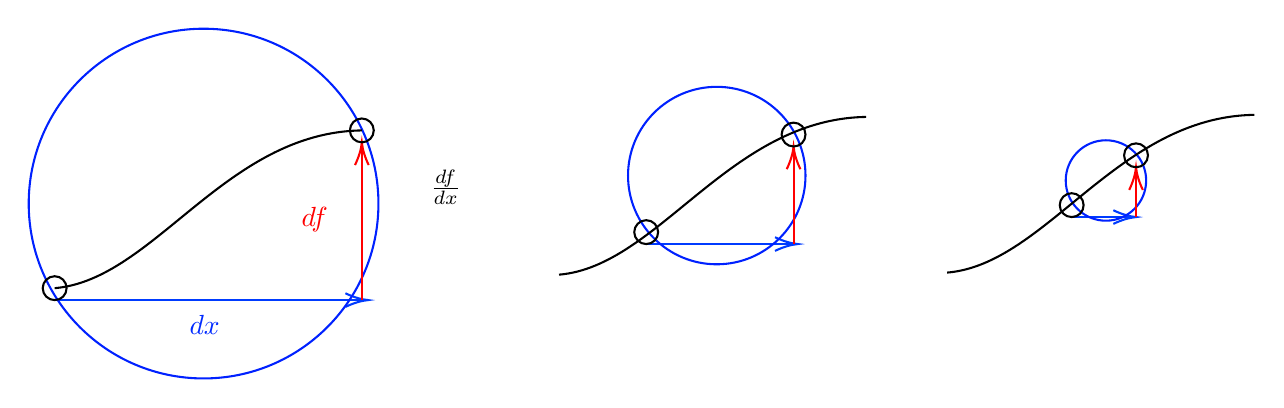
\begin{tikzpicture}[x=0.75pt,y=0.75pt,yscale=-1,xscale=1]
%uncomment if require: \path (0,300); %set diagram left start at 0, and has height of 300

%Straight Lines [id:da7431716710742607] 
\draw [color={rgb, 255:red, 0; green, 59; blue, 255 }  ,draw opacity=1 ]   (326.5,175.75) -- (397.5,175.75) ;
\draw [shift={(399.5,175.75)}, rotate = 180] [color={rgb, 255:red, 0; green, 59; blue, 255 }  ,draw opacity=1 ][line width=0.75]    (10.93,-3.29) .. controls (6.95,-1.4) and (3.31,-0.3) .. (0,0) .. controls (3.31,0.3) and (6.95,1.4) .. (10.93,3.29)   ;
%Shape: Circle [id:dp9644160811796276] 
\draw  [color={rgb, 255:red, 0; green, 33; blue, 255 }  ,draw opacity=1 ] (317.75,142.75) .. controls (317.75,119.14) and (336.89,100) .. (360.5,100) .. controls (384.11,100) and (403.25,119.14) .. (403.25,142.75) .. controls (403.25,166.36) and (384.11,185.5) .. (360.5,185.5) .. controls (336.89,185.5) and (317.75,166.36) .. (317.75,142.75) -- cycle ;
%Curve Lines [id:da3240856205395106] 
\draw    (284.5,190.5) .. controls (332.5,186.5) and (366.5,115.5) .. (432.5,114.5) ;
%Straight Lines [id:da874388198033234] 
\draw [color={rgb, 255:red, 255; green, 0; blue, 0 }  ,draw opacity=1 ]   (397.5,175.75) -- (397.5,130.75) ;
\draw [shift={(397.5,128.75)}, rotate = 450] [color={rgb, 255:red, 255; green, 0; blue, 0 }  ,draw opacity=1 ][line width=0.75]    (10.93,-3.29) .. controls (6.95,-1.4) and (3.31,-0.3) .. (0,0) .. controls (3.31,0.3) and (6.95,1.4) .. (10.93,3.29)   ;
%Straight Lines [id:da45029407338403327] 
\draw [color={rgb, 255:red, 0; green, 59; blue, 255 }  ,draw opacity=1 ]   (531.5,162.75) -- (560.5,162.75) ;
\draw [shift={(562.5,162.75)}, rotate = 180] [color={rgb, 255:red, 0; green, 59; blue, 255 }  ,draw opacity=1 ][line width=0.75]    (10.93,-3.29) .. controls (6.95,-1.4) and (3.31,-0.3) .. (0,0) .. controls (3.31,0.3) and (6.95,1.4) .. (10.93,3.29)   ;
%Shape: Circle [id:dp6907913190401643] 
\draw  [color={rgb, 255:red, 0; green, 33; blue, 255 }  ,draw opacity=1 ] (528.63,145.13) .. controls (528.63,134.42) and (537.3,125.75) .. (548,125.75) .. controls (558.7,125.75) and (567.38,134.42) .. (567.38,145.13) .. controls (567.38,155.83) and (558.7,164.5) .. (548,164.5) .. controls (537.3,164.5) and (528.63,155.83) .. (528.63,145.13) -- cycle ;
%Curve Lines [id:da7813152440439562] 
\draw    (471.5,189.5) .. controls (519.5,185.5) and (553.5,114.5) .. (619.5,113.5) ;
%Straight Lines [id:da4446042787516894] 
\draw [color={rgb, 255:red, 255; green, 0; blue, 0 }  ,draw opacity=1 ]   (562.5,162.75) -- (562.5,140.75) ;
\draw [shift={(562.5,138.75)}, rotate = 450] [color={rgb, 255:red, 255; green, 0; blue, 0 }  ,draw opacity=1 ][line width=0.75]    (10.93,-3.29) .. controls (6.95,-1.4) and (3.31,-0.3) .. (0,0) .. controls (3.31,0.3) and (6.95,1.4) .. (10.93,3.29)   ;
%Straight Lines [id:da8689576118431565] 
\draw [color={rgb, 255:red, 0; green, 59; blue, 255 }  ,draw opacity=1 ]   (41.5,202.75) -- (190.5,202.75) ;
\draw [shift={(192.5,202.75)}, rotate = 180] [color={rgb, 255:red, 0; green, 59; blue, 255 }  ,draw opacity=1 ][line width=0.75]    (10.93,-3.29) .. controls (6.95,-1.4) and (3.31,-0.3) .. (0,0) .. controls (3.31,0.3) and (6.95,1.4) .. (10.93,3.29)   ;
%Shape: Circle [id:dp15051410322467185] 
\draw  [color={rgb, 255:red, 0; green, 33; blue, 255 }  ,draw opacity=1 ] (29,156.25) .. controls (29,109.72) and (66.72,72) .. (113.25,72) .. controls (159.78,72) and (197.5,109.72) .. (197.5,156.25) .. controls (197.5,202.78) and (159.78,240.5) .. (113.25,240.5) .. controls (66.72,240.5) and (29,202.78) .. (29,156.25) -- cycle ;
%Curve Lines [id:da20936258103749295] 
\draw    (41.5,197) .. controls (89.5,193) and (123.5,122) .. (189.5,121) ;
%Straight Lines [id:da8584771026489159] 
\draw [color={rgb, 255:red, 255; green, 0; blue, 0 }  ,draw opacity=1 ]   (189.5,202.75) -- (189.5,128.75) ;
\draw [shift={(189.5,126.75)}, rotate = 450] [color={rgb, 255:red, 255; green, 0; blue, 0 }  ,draw opacity=1 ][line width=0.75]    (10.93,-3.29) .. controls (6.95,-1.4) and (3.31,-0.3) .. (0,0) .. controls (3.31,0.3) and (6.95,1.4) .. (10.93,3.29)   ;
%Shape: Circle [id:dp7775919650361445] 
\draw   (35.75,197) .. controls (35.75,193.82) and (38.32,191.25) .. (41.5,191.25) .. controls (44.68,191.25) and (47.25,193.82) .. (47.25,197) .. controls (47.25,200.18) and (44.68,202.75) .. (41.5,202.75) .. controls (38.32,202.75) and (35.75,200.18) .. (35.75,197) -- cycle ;
%Shape: Circle [id:dp8539055538820641] 
\draw   (183.75,121) .. controls (183.75,117.82) and (186.32,115.25) .. (189.5,115.25) .. controls (192.68,115.25) and (195.25,117.82) .. (195.25,121) .. controls (195.25,124.18) and (192.68,126.75) .. (189.5,126.75) .. controls (186.32,126.75) and (183.75,124.18) .. (183.75,121) -- cycle ;
%Shape: Circle [id:dp7979709638068112] 
\draw   (320.75,170) .. controls (320.75,166.82) and (323.32,164.25) .. (326.5,164.25) .. controls (329.68,164.25) and (332.25,166.82) .. (332.25,170) .. controls (332.25,173.18) and (329.68,175.75) .. (326.5,175.75) .. controls (323.32,175.75) and (320.75,173.18) .. (320.75,170) -- cycle ;
%Shape: Circle [id:dp13691653624108513] 
\draw   (391.75,123) .. controls (391.75,119.82) and (394.32,117.25) .. (397.5,117.25) .. controls (400.68,117.25) and (403.25,119.82) .. (403.25,123) .. controls (403.25,126.18) and (400.68,128.75) .. (397.5,128.75) .. controls (394.32,128.75) and (391.75,126.18) .. (391.75,123) -- cycle ;
%Shape: Circle [id:dp5213902945692483] 
\draw   (525.75,157) .. controls (525.75,153.82) and (528.32,151.25) .. (531.5,151.25) .. controls (534.68,151.25) and (537.25,153.82) .. (537.25,157) .. controls (537.25,160.18) and (534.68,162.75) .. (531.5,162.75) .. controls (528.32,162.75) and (525.75,160.18) .. (525.75,157) -- cycle ;
%Shape: Circle [id:dp7290171817227076] 
\draw   (556.75,133) .. controls (556.75,129.82) and (559.32,127.25) .. (562.5,127.25) .. controls (565.68,127.25) and (568.25,129.82) .. (568.25,133) .. controls (568.25,136.18) and (565.68,138.75) .. (562.5,138.75) .. controls (559.32,138.75) and (556.75,136.18) .. (556.75,133) -- cycle ;

% Text Node
\draw (159,156.4) node [anchor=north west][inner sep=0.75pt]  [color={rgb, 255:red, 255; green, 0; blue, 0 }  ,opacity=1 ]  {$df$};
% Text Node
\draw (105,208.4) node [anchor=north west][inner sep=0.75pt]  [color={rgb, 255:red, 0; green, 42; blue, 255 }  ,opacity=1 ]  {$dx$};
% Text Node
\draw (221,138.4) node [anchor=north west][inner sep=0.75pt]    {$\frac{df}{dx}$};


\end{tikzpicture}
